% Chapter 7

\begin{savequote}[\quotewidth]

\qauthor{Shark}
\end{savequote}

\chapter{SFC×GC for the determination of FAMEs and PAHs in diesel fuel.} % Main chapter title
\label{Chapter7} % For referencing this chapter elsewhere, use \ref{Chapter7}

\section{Introduction}

In South Africa the quality of biodiesel is regulated by the technical standard
SANS 1935, and petrodiesel by SANS 342. There is a considerable overlap in the
requirements of the two, as discussed in Section \ref{sec:Comparison},
illustrated in Figure \ref{fig:Venn}.

The prescribed method  EN 14078 has some problems with interference \autocite{Pinho2014} \todo{amplify}. 

Polycyclic aromatic hydrocarbons (PAHs) are noxious pollutants, and are therefore regulated. 

ASTM D5168 is an SFC method for determining

\section{Experimental}

\section{The study of biodiesel blends by SFC×GC}

\subsection{Introduction}
Biodiesel can be blended in all proportions with diesel obtained from petroleum
(\keyword{petrodiesel}). The volatility of biodiesel is slightly lower than that
of petrodiesel, but in 1D gas chromatography the peaks of biodiesel compounds
with higher volatility overlap significantly with the peaks of petrodiesel
compounds of lower volatility. The high complexity of the petrodiesel therefore
interferes with the determination of the biodiesel compounds. One example of an
attempt to overcome this problem is the use of a highly polar ionic liquid
column, which increases the retention of the FAMEs in the blend relative to the
retention of the petrodiesel hydrocarbons \autocite{Ragonese2009}.

On a polar stationary phase like bare silica with a non-polar mobile phase
like carbon dioxide, the hydrocarbons from petrodiesel are not expected to be
significantly retained. But, as shown in the in the previous section, under such
conditions FAMEs are retained and separated. When we inject a blend of biodiesel
and petrodiesel on SFC×GC, we therefore expect the biodiesel portion to be
completely separated from the petrodiesel portion.

\subsection{Sample}

A B50 biodiesel blend was prepared by mixing equal volumes of biodiesel and
petrodiesel in the laboratory. The biodiesel sample was donated by a commercial
testing laboratory and had been produced from waste cooking oil by an anonymous
producer. The petrodiesel sample (Shell Extra Diesel 500 ppm) was obtained from
a consumer filling station. The injection system described in Section
\ref{sec:SFCInjection} was used to inject a \SI{0.5}{\micro\litre} volume of
this undiluted B50 blend.

\subsection{SFC}

The SFC used neat carbon dioxide at \SI{200}{\bar} inlet pressure as mobile
phase. The column consisted of five HPLC bare silica columns
(\SI{150}{\milli\metre} $\times$ \SI{4.6}{\milli\metre}, 3 $\mu$m particles)
(Restek, Pinnacle DB Silica) connected in series.

\subsection{Modulation}

The SFC eluate fractions of \SI{2}{\second} were collected on the GC column
cooled to a temperature of \SI{-20}{\celsius}. The inlet vent was held closed
for \SI{4}{\second}, and then opened for \SI{1}{\second} to release excess
pressure.

\subsection{GC}

The column used in the fast gas chromatograph was an OV-5 column, which has a
stationary phase comprised of \SI{5}{\percent} diphenyl, \SI{95}{\percent}
dimethylpolysiloxane. It was \SI{1}{\metre} long, with an internal diameter of
\SI{0.25}{\milli\metre}. The thickness of the stationary phase was
\SI{0.25}{\micro\metre}.

The temperature was ramped from \SI{-20}{\celsius} at a rate of
\SI{1800}{\celsius\per\minute} to \SI{250}{\celsius}, where it was maintained
for \SI{6}{s}. After the temperature program had ended the column was cooled to
\SI{-20}{\celsius} again and the next fraction was collected.

The detector was an FID at \SI{250}{\celsius}. The FID response was recorded,
and so a total of 371 fast GC chromatograms were collected to compile the 2D
chromatogram.

\subsection{Results and discussion}
\label{sec:B50Discuss}
\begin{figure}
	\centering
	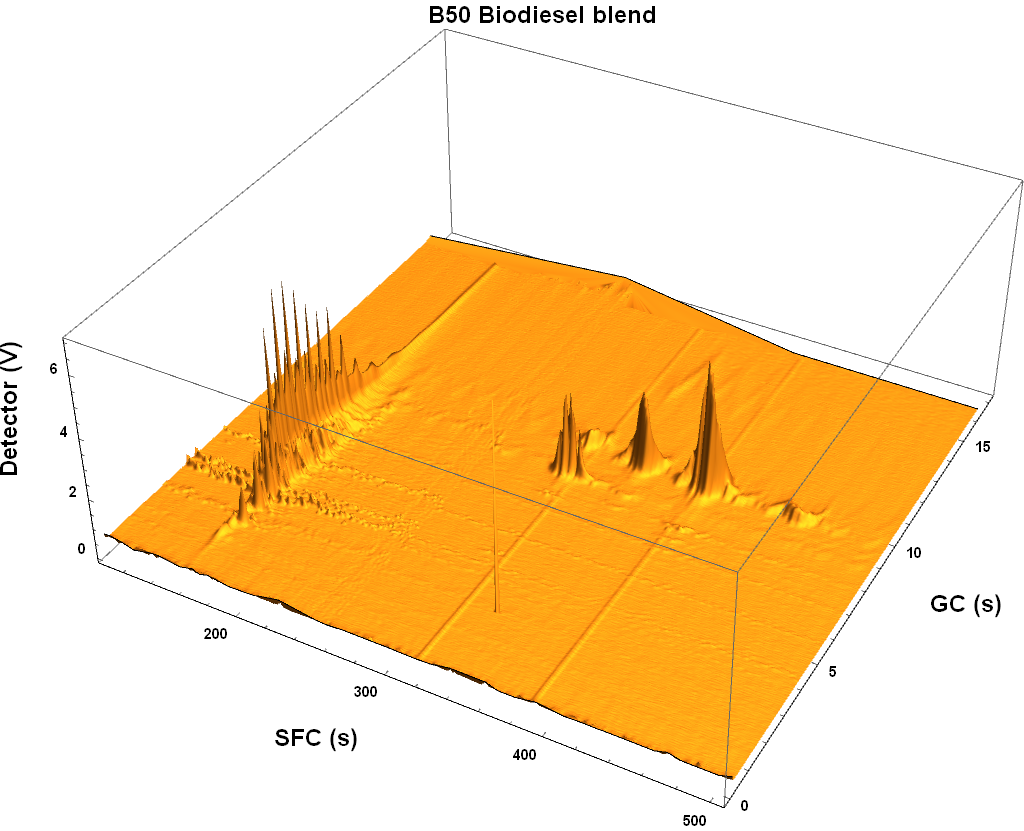
\includegraphics[width=\textwidth]{Figures/B50.png}
	\decoRule	
	
\caption[Biodiesel separated from petrodiesel.]{The separation of the biodiesel
and petrodiesel in a \SI{50}{\percent} blend. SFC: Neat CO\textsubscript{2} at
200 bar on Restek Pinnacle DB Silica column, 5 × \SI{150}{\milli\metre} ×
\SI{4.6}{\milli\metre}, \SI{3}{\micro\metre} particles. GC: Hydrogen carrier on
OV-5 \SI{1}{\metre} × \SI{0.25}{\milli\metre} × \SI{0.25}{\micro\metre},
temperature program \SI{-20}{\celsius} to \SI{250}{\celsius} at
\SI{1800}{\celsius\per\minute} hold for \SI{6}{\second}. GC runs: 371.}

	
	\label{fig:B50} 
\end{figure}

The chromatogram of the biodiesel/petrodiesel blend (Figure \ref{fig:B50}) shows
that the blend was separated into two distinct groups of compounds. At a \oneD
(SFC) retention time of about \SI{160}{\second} the hydrocarbons from the
petrodiesel part of the blend elutes. To those familiar with petrochemical
chromatography the characteristic unresolved complex mixture (``hydrocarbon
hump'') topped by alkane peaks will be instantly recognizable as representing
a petroleum product. (See Figure \ref{fig:HCHump} for an example.)


\begin{figure}
	\centering
	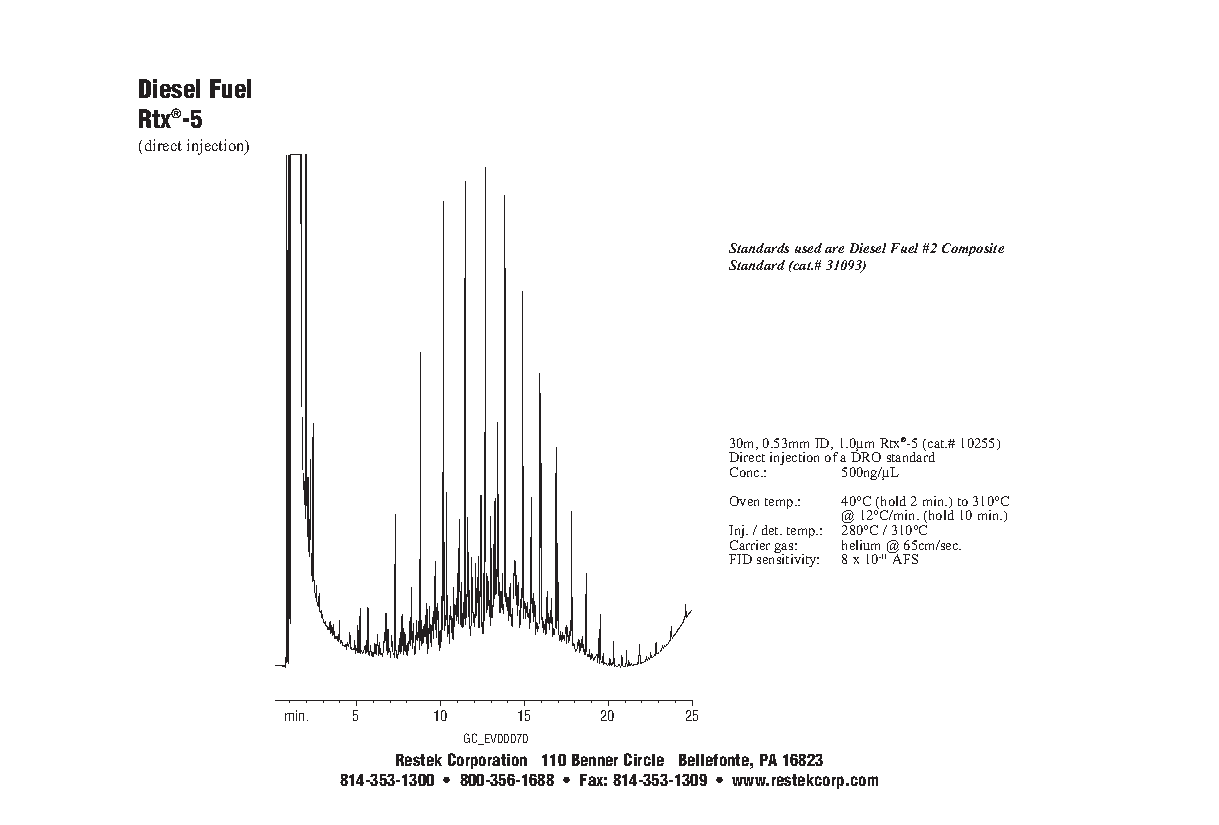
\includegraphics[width=\textwidth]{Figures/hchump.pdf}
	\decoRule	
	
\caption[An example of a petrochemical fuel chromatogram.]{An example of a GC
chromatogram obtained from a petroleum-based diesel fuel sample, showing the
unresolved complex mixture topped by alkane peaks.}
	
	\label{fig:HCHump} 
\end{figure}

Between the \textsuperscript{1}D retention times of \SI{300}{\second} and
\SI{480}{\second} the peaks of the FAMEs are seen, clearly separated by number
of double bonds in the SFC dimension, and by volatility in the GC dimension.
When compared to Figure \ref{fig:2DSunflower}, one can surmise that the
feedstock for the biodiesel was waste sunflower oil.

It is worth pointing out that the hydrocarbons from the petrodiesel fraction of
the blend were also separated on the SFC dimension \autocite{Venter1999a}. This
is not surprising: the standard ASTM D 5186 provides a method for the
determination of aromatic compounds in diesel by SFC \autocite{ASTMD5186}. The
application of this method separates the unretained non-aromatics from the
monoaromatics and from the polynuclear aromatics. The SFC×GC method provides
additional information about the volatility of those aromatics which could help
to quantify or identify them, but that falls outside the scope of this
discussion.

This separation shows that SFC×GC can be used to investigate the biodiesel
component of petrodiesel/biodiesel blends without sample pre-treatment or
specialized columns. The intrinsic orthogonality provides easy identification of
components and the excess separation space allows for the addition of suitable
internal standards for reliable qualitative and quantitative analysis with the
robust FID with its predictable response. Expensive
mass spectrometric detection is unnecessary

Being able to determine the biodiesel content of biodiesel blends may prove
useful in at least two scenarios: 

The first is in monitoring blending. Biodiesel, essentially a mixture of esters,
is quite polar compared to petrodiesel, essentially a mixture of hydrocarbons.
This means that blending might not be a matter of just pumping the relevant volumes
of the respective fuels into a tank and relying on diffusion to complete the
mixing. Being able to determine the amount of biodiesel in different samples of
a blend will provide assurance that the blend is homogenous and should perform
according to expectations. While such a test is perhaps better performed using a
spectroscopic method, SFC×GC can provide information for calibration, and will
of course be invaluable during trouble shooting.

The second application of SFC×GC is in regulating biodiesel content. In some
political environments fuels might be taxed according to their
biologically-derived content, for example to promote agriculture or to meet
carbon emissions targets. Sometimes biological content is not encouraged by
taxation, but simply mandated. Such incentives and mandates are of course liable
to corruption, and therefore the ability to monitor the blending of the fuels is
needed. The most reliable way to differentiate between organic matter derived
from biological sources and organic matter derived from fossil sources is a
radiochemical method, where the content of radioactive \textsuperscript{14}C is
determined. (Organic material from fossil sources contains no
\textsuperscript{14}C.) The technical standard ASTM D6866 provides an approved
method. But radiochemical methods require specialized equipment and trained
staff, whereas fuel laboratories more often have experience with chromatographic
techniques and might find SFC×GC a useful technique to provide evidence that a
diesel fuel blend contains the stated amount of biodiesel.



\section{Results}


\section{Discussion}


\section{Conclusion}

\todos